\chapter{多视角投影结合隐函数的点云重建方法}
从点云数据重建出完整的表面是许多几何相关应用的关键步骤,例如虚拟换装,自由视角渲染等。随着扫描设备的普及,从专业的3D扫描仪到消费级深度传感器如微软的Kinect,再到如今最新的手机上的深度摄像头,获取点云的途径变得多样。正因如此,点云的质量水平也随着设备不同而差异巨大,反观点云重建的算法能达到的效果仍然有提高空间。原始点云的随机噪声、非均匀采样以及遮挡空洞等问题,都是重建算法应该解决的问题。根据是否基于数据驱动提取先验知识,可以将点云重建的已有研究工作分为两类。

\citet{berger17}撰写了关于传统点云重建的详尽综述,根据假设的不同、噪声的种类以及输出的表达形式对方法进行了分类与比较。\citet{digne11}通过连续迭代曲率的方法对点云进行平滑操作并三角化,\citet{OHRHALLINGER2013645}通过优化三角面片的最长边之和来求解稀疏点云的表面,然而这些方法对噪声十分敏感。除了这类组合优化的思路,另一类方法从一个初始的参数化模板开始变形,逐渐逼近点云数据。\citet{sharf06}以单位球为起点将其置于点云的内部,一边变形一边细分,以此渐进拟合到点云。\citet{li10}用一维的骨骼参数化模型拟合线状结构,来处理比较细的结构。这类方法往往受到模板的限制,无法改变拓扑结构,当点云的拓扑与模板有明显差异时,拟合结果较差。为了对抗噪声同时能够处理任意的拓扑关系,许多方法用隐函数来表达几何,通过拟合点云求解出隐函数,最后从中提取水平集(Level set)作为表面。\citet{hoppe92}首次引入了这套方法,隐函数作为几何表达形式的想法开始受到广泛关注,探讨隐函数本身表达的方法开始出现,包括频域上的傅里叶系数\citet{kazhdan05}和小波变换\citet{manson08},\citet{ohtake05}在多尺度的层级模型下利用径向基函数(RBF,radial basis functions),提高了非均匀采样情形下的重建效果。\citet{alliez07}利用点云的维诺图(voronoi diagram)和主成分分析(PCA)来对隐函数梯度进行建模,通过求解系统的特征值(SVD)对隐函数进行拟合。而在以隐函数为基础的这类方法中,泊松重建\citep{kazhdan2013, kazhdan2006}具有绝对的优势。它以点云的位置信息和法向信息作为输入,约束重建后的表面要逼近点云,同时表面的法向与点云的法向保持一致。但由于所有的分析仅基于输入数据本身,没有任何额外先验,重建出的表面往往过于平滑且缺少细节,针对噪声和空洞的补全往往是不正确的。更糟糕的是,大多数情况下输入点云的法向需要从点云本身去计算,这个过程本身对噪声和采样密度就十分敏感,这无疑放大了噪声的影响从而大大限制了重建出的几何质量。

最近,数据驱动的点云重建方法有了进展,这些方法试图从一定规模的数据集中学到集合的先验。\citet{ladicky17}使用回归森林(regression forest)来从点云数据预测空间任意点到表面的距离(SDF,signed distance function),并使用八叉树和GPU加速。后来的方法倾向于用一个全局特征向量来表达整个几何,一般使用神经网络编码器从点云数据中获得。对于给定的数据集,特征向量一般在高维空间中存在结构化的分布,因此网络从中学到的信息就可以用来作为一类几何的先验。隐函数在空间离散后形成三维网格,一般为固定分辨率,隐函数的值存储在各个格点上。\citet{ogn2017}用八叉树来减少离散网格的存储开销,仅仅子啊叶子节点上使用卷积网络进行隐函数的预测。\citet{groueix2018}以固定分辨率的二维平面作为参数化模板,使用多歌不同参数的模板单体一起来拼成整个表面,具有较好的泛化性能。最新的工作抛弃了空间离散化的形式,转而使用神经网络来直接表达连续的隐函数\citep{chen19, meshcheder2019cvpr, park2019cvpr},将空间中的任意点映射成隐函数值,这样的表达不再受到离散网格的分辨率影响,适合表达具有复杂拓扑结构的表面,理论上能够取得任意的精度。

本章的点云重建方法在此基础上,取隐函数为几何表达形式,结合新的点云编码方法进行点云重建。对于带噪声和非均匀采样的点云,甚至是由于遮挡造成空洞的人体扫描点云,新方法都能重建出细节丰富的完整模型,保留诸如衣服褶皱等几何细节,同时能正确处理不同拓扑的情况。新方法的核心思想在于对点云的结构化处理,先将点云渲染到多个视角得到深度图,再用编码器将点云图映射到特征空间。隐函数由多层感知机(MLP,multilayer perceptron)实现,对于空间中任意点,通过投影到各个视角上取得点云的特征,经过融合后由隐函数映射成表达该点位于几何内部还是外部的概率,整体算法框架如图\ref{fig:pc_pipeline}所示。
\begin{figure}[!htbp]
    \centering
    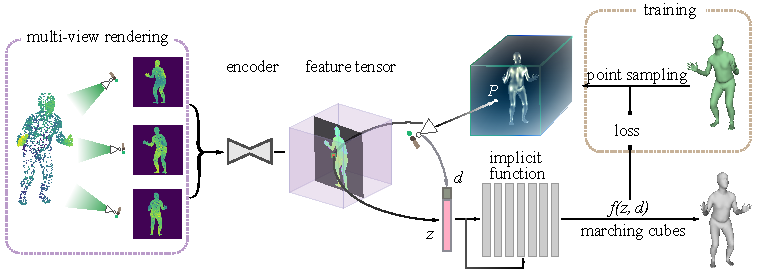
\includegraphics[width=\textwidth]{pipeline_pc.pdf}
    \bicaption[算法框架图]{算法框架图。对于输入点云,经过多视角投影和特征提取后,给定空间点$P$,投影到各个视角中得到特征向量$z$,连同投影得到的深度$d$,经过隐函数得到位于表面几何内/外部的概率$f(z, d)$,提取等值面后得到输出三角面片。}[Pipeline of pointcloud reconstruction]{Pipeline of pointcloud reconstruction. After multi-view projection and feature extraction, a 3D point $P$ is projected to each view to get the feature vector $z$ and the depth $d$, the implicit function predicts the inside/outside probability. The surface is extracted using marching cubes.}
    \label{fig:pc_pipeline}
\end{figure}
相比于直接用三维网格对点云进行光栅化,通过投影到二维网格的方式更加节省内存。借助基于卷积操作的特征提取过程,可以在多个尺度上对点云进行去噪和空洞补全。通过在两个人体数据集上的实验,新方法可以生成更加精确和富有细节的点云重建结果。主要的贡献包括:提出了结合隐函数与数据驱动的点云重建算法。利用端到端的可导过程表达点云到表面几何的生成,能从已有的数据中学习处理点云噪声和空洞的知识,提升点云重建的质量和鲁棒性;结合可渲染和基于卷积的编码器对点云作结构化处理,节省内存地同时对点云进行了去噪和补洞操作,同时新算法能够处理任意数量的视角,可扩展性极强。

\section{隐函数的几何建模过程}
将真实的几何表面记作$M$,点云数据$P=\{p_1, \dots, p_N\}$从其上采样得到,采样过程中设备噪声会叠加到点云的位置上,视角变化和自遮挡也会造成空洞。$M$可以表达为函数$F(\cdot)$的等值面,如公式(\ref{eq:pc_1})所示。函数$F(\cdot)$一般表示$M$的有向距离场(SDF,signed distance function)。
\begin{equation} \label{eq:pc_1}
    \adddotsbeforeeqnnum%
    M = \{x \in \mathbb{R}^3 | F(x) = 0\}
\end{equation}

对于空间中任意一点$x$,引入内嵌函数$h(\cdot)$表示将其映射成高维特征向量,以及函数$f(\cdot)$将高维特征向量映射成SDF的值,则将两个函数进行级联,用来近似$F(\cdot)$,如公式(\ref{eq:pc_2})所示。该分解过程与深度学习任务中常见的编解码器结构(encoder-decoder structure)相对应。
\begin{equation} \label{eq:pc_2}
    \adddotsbeforeeqnnum%
    F(x) \approx f(h(x))
\end{equation}

在$M$所在的欧式空间中采样点集$X = \{x_1, x_2, \dots, x_N\}$,且其对应的SDF值为$Y=\{y_1, y_2, \dots, y_N\}$,则$M$与隐函数$F(\cdot)$的关系可以由公式(\ref{eq:pc_loss})所表达的损失函数表示。理论上,采样点数趋于无穷且损失函数值接近零时,隐函数便精确地表达了表面。
\begin{equation} \label{eq:pc_loss}
    \adddotsbeforeeqnnum%
    L = \sum_{i=1}^N \|f(h(x_i)) - y_i\|^2
\end{equation}

以上的过程中包含三个步骤,包括从点云中获取并推测几何特征信息、点集$X$的采样方法以及到SDF函数的映射,每步都影响这隐函数描述表面几何的精确程度。

\subsection{基于多视角投影的点云特征提取}
采样点云的非结构性使得无论是全局信息还是局部信息的获取都十分昂贵,对于空间中的任意点,从点云中插值出尽可能准确的信息更为关键,点云本身的噪声和缺失等特性同样增加了求解的难度。采用多视角投影的方式将点云映射到多歌二维相平面,看起来每个视角在投影过程中损失了一个维度的位置信息,然而在每个视角下却得到了二维的结构话信息,查找、补全以及去噪等操作都更易于完成,多个视角的联合推理可以将之前投影损失掉的信息进行补偿,与在空间中划分三维网格,多视角投影占用存储小,速度快,同时信息密度更高。

假设点云$P=\{p_1, \dots, p_N\}$已经归一化到单位球内,在球面上均匀采样相机变换参数$T=\{t_1, \dots, t_l\}$,在每个相机下渲染点云$P$的深度图$I=\{I_1, \dots, I_l\}$,即图中的每个像素记录投影到该位置的点沿着相机z轴的距离。点的渲染采用可导渲染(differentiable rendering)的方法,在点光栅化到像素域时,让其对周围像素的影响按距离衰减。可导渲染使得点投影到多个视角中的像素之间保持了关联。

为了给渲染得到的深度图及进行编码提取特征,采用了Stacked Hourglass结构\citep{newell2016},该结构已被验证适合提取图片特征并被广泛使用。深度图$I=\{I_1, \dots, I_l\}$经过编码器后生成特征张量$Z=\{Z_1, \dots, Z_l\}$。对于空间中任意点$x_i$,给定相机$t_j$和对应的特征张量切片$Z_j$,能够通过投影和采样得到特征向量,如公式(\ref{eq:pc_4})所示。
\begin{equation} \label{eq:pc_4}
    \adddotsbeforeeqnnum%
    z_i^j = Z_j(\pi(x_i, t_j))
\end{equation}

其中函数$\pi(\cdot, \cdot)$是给定点位置坐标和相机参数之后,将点投影到相平面的变换函数。点$x_i$在所有相机里得到的向量通过融合函数$s(\cdot)$获得点的特征,$s(\cdot)$的一个自然的实现为点在所有相机里采样向量的平均值,如公式(\ref{eq:pc_5})所示。
\begin{equation} \label{eq:pc_5}
    \adddotsbeforeeqnnum%
    z_i= s(z_i^1, \dots, z_i^l)
\end{equation}

基于卷积操作的编码器能够利用局部到全局的邻域信息来提取和融合点云中不同点的关系,以及不同尺度的几何特征,同时完成补全和去噪等工作。这样的设计保证编码器对点云中几何信息的学习过程与测试时点采样的数量解耦开。如果任取的一个点是属于点云的,多视角特征保证了各个视角对点提出的特征在几何上是严格一致的,而当该点不属于点云时,提取的特征又能通过多视角约束对采样点的隐函数值进行推断。

\subsection{空间点集的采样}
对于二维流形$M$,给定空间中的采样点集$X = \{x_1, x_2, \dots, x_N\}$,可以计算出各个点SDF的值,从而通过优化公式(\ref{eq:pc_loss})来使得隐函数逼近$M$。理论上采样点数量越多逼近质量越好,但是限于计算时间和空间,需要在保证$N$比较小的前提下提高逼近效果。$M$在三维空间中的测度为零,因此按照均匀采样得到的点大部分都会离表面很远,也就无法刻画复杂的几何信息。反之倘如仅在$M$的附近采样,空间中大部分的位置就无法受到监督,容易造成过拟合。因此,点集$X$的采样需要同时考虑表面附近的情况和空间中其他位置的情况,在实现时采取了与\citet{saito2019pifu}类似的采样策略。

对于归一化到单位正方体内的表面$M$,首先在其上随机采点,随后对点增加扰动,扰动的各个分量服从正态分布$\mathcal{N}(0, 0.05)$,以此得到随机分布在表面附近的点。另一方面,在单位正方体内进行均匀采样。表面附近的采样点与均匀采样的点数量按照$16:1$来分配,这些点一同构成了采样点集。

\subsection{隐函数模块的设计}
隐函数模块$f(\cdot)$用一个MLP表达,对于点集$X=\{x_1, x_2, \dots, x_N\}$中的点$x_i$,按照如公式(\ref{eq:pc_5})中计算出特征$z_i$后,与点坐标$x_i$一起给进网络。为了平衡位置信息与几何特征的维度,以及提高隐函数对高频信息的拟合能力,在$x_i$进入隐函数网络之前,对其进行位置编码(positional encoding),利用如公式(\ref{eq:pc_6})所示的两组函数对$x_i$进行映射并组成新的向量。
\begin{equation} \label{eq:pc_6}
    \adddotsbeforeeqnnum%
    \phi_i(x) = \sin(2^i \cdot x), \psi_i(x) = \cos(2^i \cdot x)
\end{equation}

另一方面,不管是在表面内外的点,如果远离表面,SDF的计算对推断表面并没有太大意义,同时SDF函数本身的计算代价也不低。仅仅需要判断$x_i$是在面的外部还是内部,就足以通过提取内外部的边界得到表面几何。因此隐函数模块可以进一步简化为求解二分类问题。

\section{数据准备与模型训练}
整个框架中需要训练的模块只有点云深度图的编码器与表达隐函数的MLP模块,参数的学习需要准备大量的数据。常见的数据集以三角面片的形式存储,因此在准备训练数据的时候需要对模型进行挑选和生成训练标签。为了处理实际情况中的噪声,需要在训练数据中模拟生成各类噪声。

\subsection{训练数据的生成}
一组训练数据应包括输入点云与真实模型,根据公式(\ref{eq:pc_loss})的损失函数,真实模型又是由采样点集与点的内外部二分类标签所表达。给定一个三角面片模型,首先从面上尽可能均匀地采样出点云。接着按照空间点集的采样方法采出包括面附近以及空间中均匀分布的点集,然后对每个点通过光线追踪测试位于模型的内部还是外部,如图\ref{fig:pc_inout}。值得注意,这里提到的采样得到的点云数据和采样点集容易混淆,从模型上采点云是为了模拟输入数据,而采点集是为了训练隐函数来逼近真实模型。
\begin{figure}[!htbp]
    \centering
    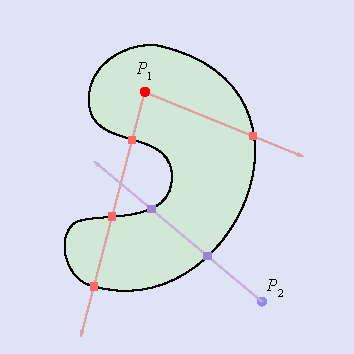
\includegraphics[width=0.5\textwidth]{inner_outer_pc.pdf}
    \bicaption[采样点的位置测试]{采样点的位置测试。自位于模型内部的采样点发出测试光线,与模型交点的个数一般为奇数,除非出现至少以此相切的情况;而自模型外部的采样点发出测试光线,与模型交点的个数一般为偶数}[Position test for sample points]{Position test for sample points. The number of intersection of the mesh boundary  and a ray emitted from an inner point should be odd, and the number of intersection of the mesh boundary and a ray emitted from a outer point should be even}
    \label{fig:pc_inout}
\end{figure}

编码器的输入是点云渲染到多个视角的深度图,因此在训练时可以将渲染过程进行预处理,以节省训练时间。对每个模型在单位球上采样270个相机位置,并渲染相应视角的点云深度图,为了保持深度图的浮点精度,采用EXR格式存储深度图文件。这样做还可以使得在训练来自一个点云不同视角的投影时,可以多次采样模型的测试点集和分类标签,使得单个模型有了更多的点集采样,有助于隐函数模块对真实几何的逼近。

\subsection{点云噪声的模拟}
与实际场景中扫描得到的真实点云相比,从三角面片上采样得到的点云不仅采样均匀,而且没有噪声和遮挡造成的空洞,在这样的数据上训练出的隐函数模块对真实数据的响应会差很多,因此需要模拟产生出噪声并叠加到采样点云上。主要考虑三种噪声模型,首先是对点云中各个点添加位置扰动,比对实际深度传感器的噪声数据,对归一化后的点云添加了方差为0.002的高斯扰动;第二种扰动为不均匀采样,先将同一个模型的面片随机分为30组,对每组面片按照面积比例,采样不同密度的点,再把所有采样点合起来作为最终的点云;第三种噪声考虑遮挡变化造成的空洞,在每个模型上随机选取20个点,采用宽度优先搜索(BFS,breadth first search)记录点周围若干步以内的面片,并将其删去,在余下的模型上再采样点云。图\ref{fig:pc_hole} 展示了步长为2时面片搜索的示例。
\begin{figure}[!htbp]
    \centering
    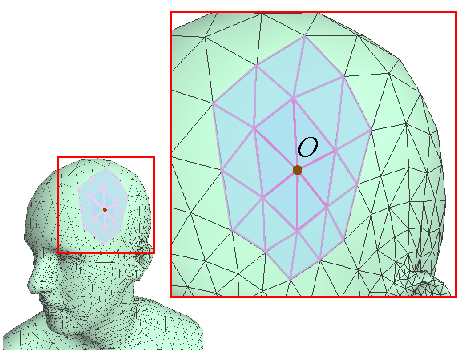
\includegraphics[width=0.6\textwidth]{hole_pc.pdf}
    \bicaption[面片上空洞的模拟]{面片上空洞的模拟。点$O$为采样的中心点,以两步为例,标识出了可达区域内的面片。}[Simulation of hole on the mesh]{Simulation of hole one the mesh. $O$ is one of the random samples. If the step number is two, the accessible triangles are marked.}
    \label{fig:pc_hole}
\end{figure}

\subsection{网络的训练与测试}
由于对点云的深度图进行了预渲染,训练的第一阶段仅包含单视角情况。一组训练数据就包含单视角的点云深度图、相机参数、对应模型的采样点集和各点的二分类标签。编码器对深度图进行编码,采样点投影到深度图得到插值的特征向量,并利用隐函数预测二分类的结果。在单视角训练结束之后,才进行多视角的数据进行调优,调优过程只需要2--3轮迭代就能收敛到较好的结果。这种渐进式增加视角数量的策略,提高了训练效率和泛化性能。

在测试的时候,对于输入点云,投影过程与训练过程无异。差异在于点采样的方式,由于测试时的目标是最终提取出面片,因此测试时按照规则三维网格进行采样。给定网格分辨率后对每个格点进行投影、采样特征向量以及预测隐函数值的过程,最终就可以通过marching cubes等方式提出面片。为了提高网格的预测效率,可以采用八叉树加速,对当前层级八个顶点分类结果一样的体素,就无须再继续细分下去,当然这样的剪枝有一定概率会在粗粒度时将整个几何丢失。

\section{本章小结}
本章介绍了以隐函数表达几何的同时基于多视角投影的点云重建算法部分。点云经投影和编码后得到特征,空间中的任意点从点云的特征上插值出自己的特征向量,代表隐函数的MLP继而将特征向量映射成隐函数值。训练过程中,特殊的点集采样策略提高了隐函数的逼近效果,并且通过模拟叠加噪声来提高鲁棒性,而两阶段渐进增加视角数量的策略缩减了训练时间。